\chapter{面向熟练者的拼音输入法设计}
  \section{设计初衷}

  大多数18到30岁左右用户都受过良好的教育,拼音基础知识牢固,已经有十年以上的拼音输入法使用经验,并且能够熟练地使用除基础输入以外更多新增特性。(见第\ref{sec:new_feature}节)在上一章的讨论中,我们把这一部分用户列为非初学者用户,不妨称其为熟练者。由于熟练者对拼音掌握的程度远远高于初学者,我们可以假定,他们在拼音形态的辨识,拼音与汉字的匹配方面不存在任何困难。因此他们在触摸设备上的输入体验更多的局限于现有键盘的布局和交互技术。

  正如之前第\ref{sec:limit}节所讨论的一样,现有拼音输入法键盘,无论是QWERTY键盘还是九键键盘,并不是为拼音输入定制的。再者现有的拼音输入法大多采用点击输入的方式。无论单点触摸设备还是多点触摸设备,其基本的交互方式都是在屏幕同一位置按下和抬起,手指离开屏幕后才会有位移动作。事实上,触摸设备提供了更加丰富的交互体验,例如单指滑动,双指收缩等等,输入法程序并没有很好地利用起来。

  本设计主要面向熟练的拼音输入用户,目的在于克服传统键盘所带来的输入局限性,根据韵母自身的特性进行拆分,提供一种充分利用大型多点触摸设备所提供的交互功能,布局更紧凑的中文输入方法,提高中文输入效率和体验。

  \section{设计分析}
  \subsection{布局设计}

  基本的布局设计思路与面向初学者的设计类似。考虑到汉语拼音的多元音韵母形式上是由单元音韵母拼合而成,熟练者已经掌握所有多元音韵母的组成,我们考虑在韵母输入区只保留单元音韵母,单元音韵母使用简单的触摸动作输入,多元音韵母则使用滑动输入。

  \subsection{交互设计}

  一些可视化研究在触摸屏幕上使用了很多丰富的交互,包括一些图表上操作技术\supercite{sadana2014designing},通过显示用户输入位置热图来纠正用户操作\supercite{rudchenko2011text},。有些研究甚至考虑到了触摸设备两面的可操作性,来延伸交互的可能\supercite{buschek2014improving, shen2009double}。一些在输入法也在交互手段上做了创新,包括一些基于QWERTY键盘的变体\supercite{findlater2012beyond, shin2009multi},将键盘分离为负责区域和负责细节两个部分分别输入\supercite{don2010applying},移出某些容易造成误操作的键位\supercite{arif2014experimental}等等。这些思路都在某种程度上说明在输入法用户界面使用更丰富的交互手段是可行的并且是有效的。

  事实上,在英文的虚拟键盘上,轨迹输入早已出现\supercite{kristenssondiscrete, hinckley2002input, zhai2008interlaced},主要思路比较相似,都是储存用户输入轨迹,与标准轨迹计算相似程度,其中计算相似程度的算法多样。本设计沿袭了这一过程,使用了比较简单直接的相似度算法,应用在自定义的韵母输入区键盘上。

  \section{具体实现}
  \subsection{输入区布局设计}

  输入法的整体布局如图\ref{fig:layout2_background}所示。与面向初学者的布局类似,不再赘述。

  \begin{figure}[h]
  \noindent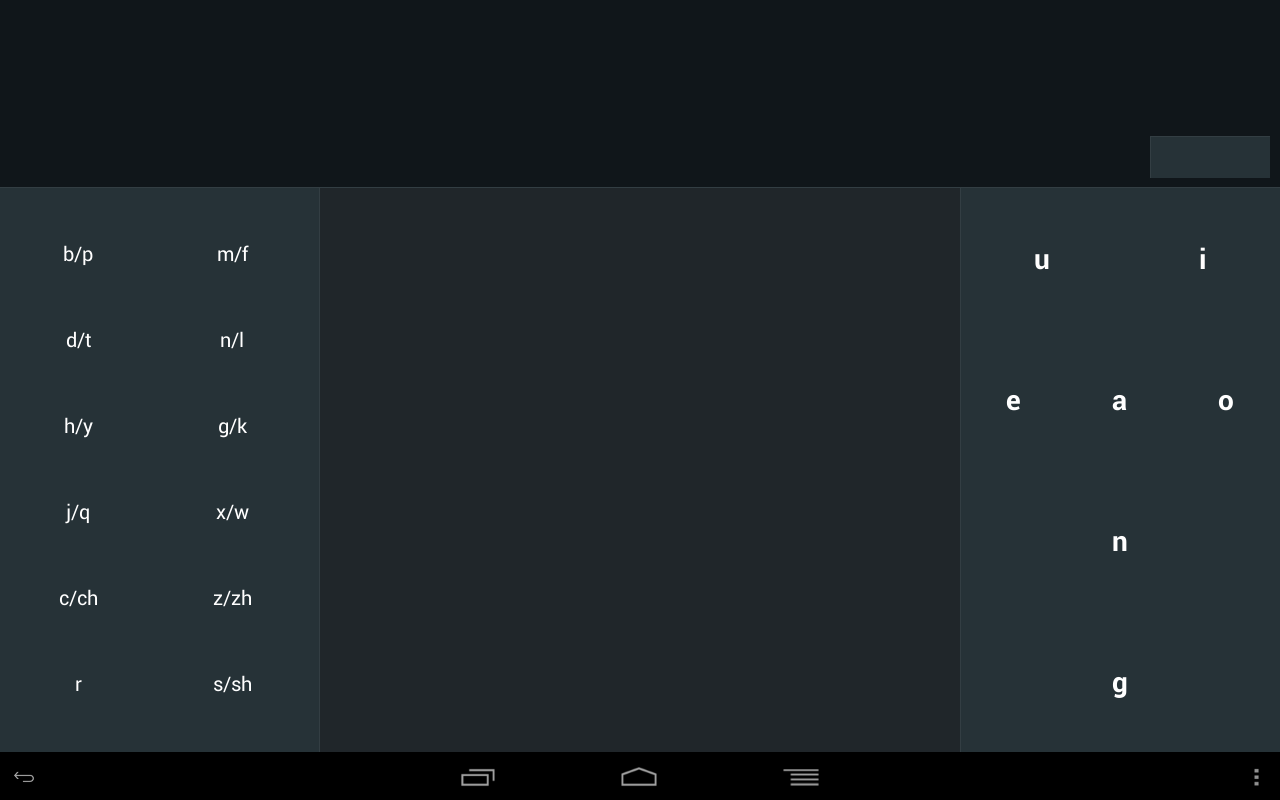
\includegraphics[width=150mm]{img/layout2_background}
  \caption{输入界面}
  \label{fig:layout2_background}
  \end{figure}

  可以看到,声母区的相邻声母进行了合并,这是为了第\ref{sec:dialect}节所做的实验性步骤,在该节有详细说明。韵母区只保留了单元音韵母,并对其排列进行了调整,使得所有其他多元音韵母都能够通过单元音组合而成,并使得其轨迹比较平滑规整。

  \subsection{输入区交互设计}

  由于声母的特殊性,无法向韵母一样拆分,故声母区的输入方式与面向初学者的没有区别。同样的,汉字备选区,汉字显示区和拼音提示区都与之前设计无差别,因此不再赘述。

  韵母区的操作分为两种:

  \begin{enumerate}
  \item
  点击:对于单元音韵母的输入,与之前的设计没有区别,直接点击对应键位即可。

  \item
  滑动:对于多元音韵母的输入,需要用户使用“滑动”这一交互手段。所谓滑动,即是在某一位置接触屏幕,保持接触并在同时移动手指,到另一位置放开手指。例如要输入 “iang” ,就需要在键位 “i” 按下,拖动手指经过 “a”,“n” 直到到达 “g”,然后放开手指。用户手指轨迹以及检索结果见图\ref{fig:layout2_input}

  \begin{figure}[h]
  \noindent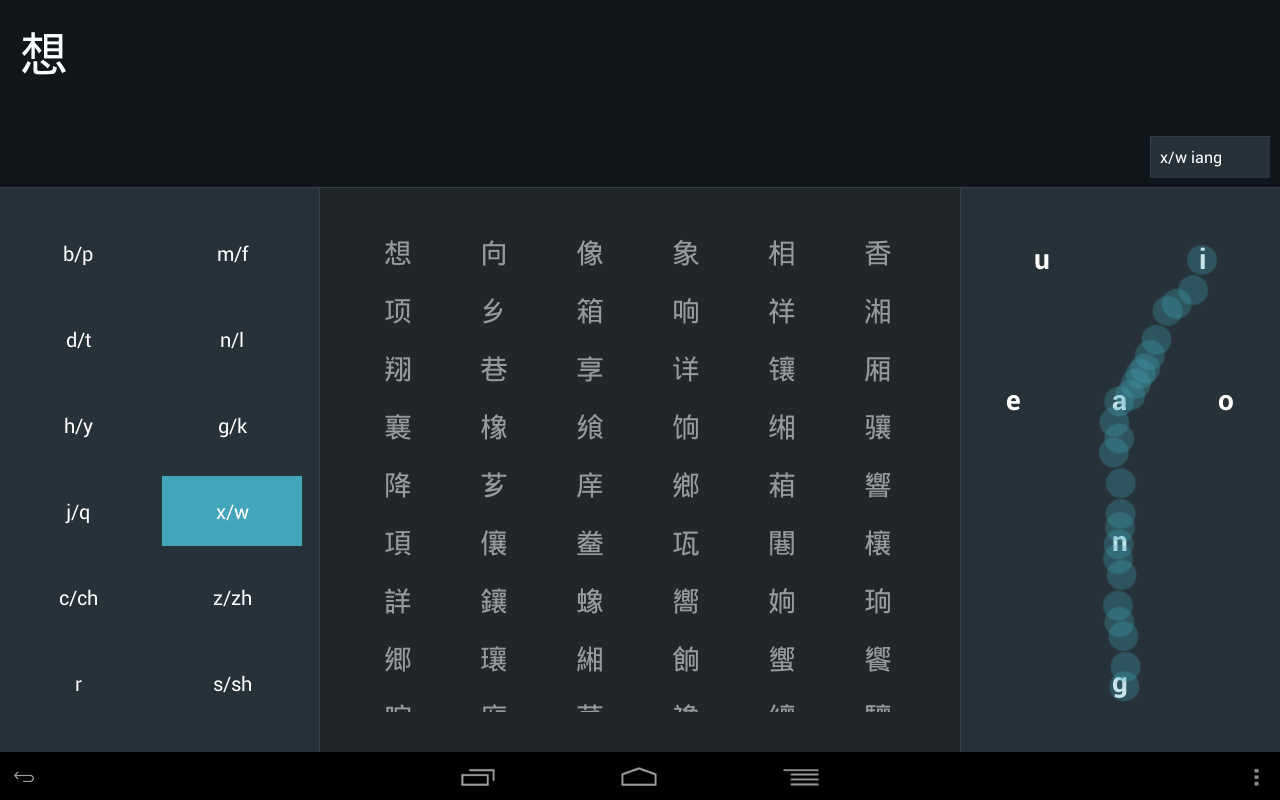
\includegraphics[width=150mm]{img/layout2_input}
  \caption{滑动输入}
  \label{fig:layout2_input}
  \end{figure}

  \end{enumerate}

  \subsection{轨迹相似度算法\label{sec:tra_algorithm}}

  本实现使用了最简单最直接的相似度算法。假设有二维平面点\(v = (x, y)\)。定义每一个单元音韵母有唯一坐标,为键位中点,得单元音韵母坐标集\(S = \{v_0, v_1, \dots, v_6\}\)。定义多元音韵母标准轨迹为其每个元音对应韵母的坐标依次连接所得的折线,即\(s = (v_{i_1}, v_{i_2}, \dots, v_{i_n}), (n \leq 6)\),其中\(I = \{i_1, i_2, \dots, i_n\}, (n \leq 6) \)为某一多元音韵母拆分成的单元音韵母在单元音韵母坐标集合中的下标。定义标准轨迹集\(S = \{s_0, s_1, \dots, s_n\}\)。

  此时,用户的滑动输入可以看做是一组点集,记为\(W\), 记点到直线距离函数为\(disL(v_1, v_2, v_3)\),表示点\(v_1\)到\((v_2, v_3)\)所在直线的欧式距离。在定义点到标准轨迹的距离:

  \[disS(v', s) = \min_{v_i \in s }\{disL(v', v_i, v_{i+1})\}\]

  由此我们定义相似度为

  \[q_i = \frac{1}{\sum_{v \in W}\,disS(v, s_i)}, (s_i \in S)\]

  相似度越大,我们认为轨迹\(W\)与标准轨迹\(s_i\)在位置上越相似,用户更倾向于选择标准轨迹为\(s_i\)的韵母。相似度最大为正无穷,即用户轨迹精准的落在标准轨迹上。

  最后,在所有相似度中求得最大的一项\(\max(q_0, q_i, \dots, q_m)\)所对应的韵母即视为用户的输入。

  算法的具体代码详见附录\ref{sec:code}。

  \subsection{本设计的优势}

  同样,考虑第\ref{sec:limit}节所提到的现有输入法的局限性,本设计的优势包括前一设计的1、2、3点以外,还有以下几点:

  \begin{enumerate}
  \item
  缩减键盘空间,使盲打成为可能:由于本设计的韵母键盘压缩了相当大的空间,使得用户可以在大型触摸设备上,双手握住设备边缘,仅靠左右手大拇指即可操作。虽然以目前的设计来看,选择汉字还是需要更多手指配合,但这已经是一大进步了。再者,由于单元音数量较少,熟练者在掌握本输入法后,在右手实现盲打的可能性较高。

  \item
  丰富交互方式,充分利用设备:在自定义韵母输入区键盘上,使用了滑动输入的方式,改进目前输入法单一的触摸交互方式。这一改善不仅充分利用了触摸设备提供的交互功能接口,还为输入法用户提供了一次新鲜的交互体验。相信随着更加完善的研究和成熟的发展,更丰富的交互手段一定会踏上输入法这一块土地。

  \end{enumerate}
